\documentclass{article}

\usepackage[margin=1.25in]{geometry}
\usepackage{listings}
\usepackage{caption}
\usepackage{color}
\usepackage{pmboxdraw}
\usepackage{amsmath}
\usepackage{graphicx}
\usepackage{siunitx}
\usepackage{cite}
\usepackage{booktabs}


\newcommand{\code}{\lstinline}
% A better code font
\usepackage{inconsolata}
\lstset{
    language=C,
    keywordstyle=\color{blue},
    basicstyle=\footnotesize\ttfamily,
    commentstyle=\color{gray},
    showstringspaces=false
}
\DeclareCaptionFont{white}{ \color{white} }
\DeclareCaptionFormat{listing}{
  \colorbox[cmyk]{0.43, 0.35, 0.35,0.01 }{
    \parbox{\textwidth}{\hspace{15pt}#1#2#3}
  }
}
\captionsetup[lstlisting]{ format=listing, labelfont=white, textfont=white, singlelinecheck=false, margin=0pt }

\begin{document}
    \tableofcontents
    \newpage

    \section{Power-On Procedures (IMPORTANT!)}
    To avoid damaging the DigiPot chip or the Arduino, circuit components must be turned on in a very particular order:
    \begin{enumerate}
        \item Turn on the power supply to the DigiPot ($\pm2.5$V). If this is the first time the circuit has been turned on in a while, check that the voltages are reasonable with a multimeter.
        \item Turn on Arduino power by plugging in the USB cable.
        \item Power on delay module to ensure grounding.
        \item Turn on opamp power ($\pm15$V) using the breadboard switch.
        \item Power lasers up (typically, to about $20$mA).
        \item Turn on photodetectors---by powering on the lasers before the detectors, we can minimize the effect of the relaxation oscillation and associated current surge.
        \item Ready
    \end{enumerate}

    \section{Project Organization}
    Figure \ref{dirform}  shows how the project is orgaized.
    \begin{itemize}
        \item The \code{data} directory contains the raw data collected.
        \begin{itemize}
            \item \code{delay} contains data on the behavior and performance of the delay modules
            \item \code{digipot} contains information on the AD5206 digital potentiometer (a chip you probably want to avoid)
            \item \code{filters} has information on the bandpass filters and their characteristics over various frequency ranges
            \item \code{lasers} has current-power curves for the three lasers in Lucas' lab. 
            \item \code{mach}\code{zehnder} has information on the response of the three MZMs.
        \end{itemize}
        \item \code{doc} has this document, and associated source files.
        \item \code{figures} has various figures and results, derived from the data. It has the same categories as the \code{data} directory.
        \begin{itemize}
            \item The \code{pinouts} directory has pinouts for the various ICs I used.
        \end{itemize}
        \item \code{manuals} has PDF manuals for the various bits used in the circuit.
        \item \code{notes} has application notes and other writeups. These also have copies in the lab notebook.
        \item \code{numericalanalysis} has my work on numerical bifurcation and theoretical prediction of the size and shape of the amplitude death region.
        \item \code{papers} has PDF copies of various relevant papers.
        \item \code{scripts} has all the Python source code for collecting and analyzing data. I'll got into more depth on what each of these scripts do later.
    \end{itemize}
    
\begin{figure}[h]
\begin{center}
\fbox{
\begin{minipage}{\dimexpr5cm\fboxsep-2\fboxrule\relax}
\noindent \code{summer-19}\\
\textSFviii\textSFvi\textSFx \code{data}\\
\textSFxi\textSFviii\textSFx\textSFx \code{delay}\\
\textSFxi\textSFviii\textSFx\textSFx \code{digipot}\\
\textSFxi\textSFviii\textSFx\textSFx \code{filters}\\
\textSFxi\textSFviii\textSFx\textSFx \code{lasers}\\
\textSFxi\textSFii\textSFx\textSFx \code{mach_zehnder}\\
\textSFviii\textSFx\textSFx \code{doc}\\
\textSFviii\textSFvi\textSFx \code{figures}\\
\textSFxi\textSFviii\textSFx\textSFx \code{delay}\\
\textSFxi\textSFviii\textSFx\textSFx \code{digipot}\\
\textSFxi\textSFviii\textSFx\textSFx \code{filters}\\
\textSFxi\textSFviii\textSFx\textSFx \code{lasers}\\
\textSFxi\textSFviii\textSFx\textSFx \code{mach_zehnder}\\
\textSFxi\textSFii\textSFx\textSFx \code{pinouts}\\
\textSFviii\textSFx\textSFx \code{manuals}\\
\textSFviii\textSFx\textSFx \code{notes}\\
\textSFviii\textSFx\textSFx \code{numericalanalysis}\\
\textSFviii\textSFx\textSFx \code{papers}\\
\textSFii\textSFx\textSFx \code{scripts}
\end{minipage}
}
\end{center}

\caption{The directory format of the project.}
\label{dirform}
\end{figure}


    \section{Data Format}
    All data is stored in the Numpy builtin compressed-archive format (\code{.npz}), since it's easy to work with in Python, makes it possible to store the data and metadata about its capture (such as time, test parameters, etc.) in the same file, and is nice and compact (no more 80MB captures!).

    \subsection{Saving and Loading}
    I've written a few utility functions to make saving and loading these files as simple as possible. Located in \code{utils.py}, the \code{save} function takes a filename, arbitrary Numpy array (any shape or dimension number), and (optionally) a dictionary of settings to save; and writes them to a file.

    Similarly, the \code{load} function, given a filename, loads that file and returns a \code{data, metadata} tuple. If the metadata is stored in a separate file (which I was doing for the first few weeks), this function loads from that instead, and resaves the data in compressed form. The code snippet below shows how to use these functions: 

    \begin{lstlisting}
import utils

data = get_data()
metadata = {
    'capname': 'Example Capture,
    'lasernum': 3,
    'lasername': 'Clara
}

utils.save("outfile", data, metadata)


# Then later, when you need the data back:

data, md = utils.load("outfile")
    \end{lstlisting}

    \subsection{Editing Files}
    The script \code{edit_md.py} can be used to modify a file's settings. Run it as
    \begin{lstlisting}
        python scripts/edit_md.py filename
    \end{lstlisting}
    and follow the instructions on the screen.

    \section{Settings}
    Various settings for the project can be found in \code{settings.py}. The first three entries in the file (\code{ROOT_DIR}, \code{FIGS_DIR}, and \code{DATA_DIR}) set the working directory, and directories to save and load figures and data from, respectively. The snippet of Python code for \code{ROOT_DIR}
    \begin{lstlisting}
        ROOT_DIR = Path(__file__).parents[1]
    \end{lstlisting}
    simply sets the root directory to the parent of the scripts directory. You shouldn't need to change any of these parameters, short of a major reorganization of the project.

    The rest of the settings are snippets from the VISA ids of various instruments used:
    \begin{itemize}
        \item The scope is a Tektronix TDS-2000C 4-channel scope w/ USB out. There's one (and only one) of these in the JLab.
        \item The function generator is an Agilent 33210A.
        \item The multimeter is an
    \end{itemize}
    I believe these snippets will be the same for any instrument of the same type, but I am not sure. If you get ``InstrumentNotFoundError'' or similar, this may be the cause.

    \section{Characterizing MZMs}

    To characterize an MZM, connect it to the associated laser, and turn on the laser power. Feed a $10\text{V}_{\text{pp}}$ triangle wave into the MZM at 8Hz. Connect channel 2 on the scope to the function generator, and channel 1 to the detector output. Run
    \begin{lstlisting}
        python scripts/MZ_getdata.py
    \end{lstlisting}
    and follow the prompts for filename and power level.

    After collecting this capture, run
    \begin{lstlisting}
        python scripts/MZ_characterize.py <filename>
    \end{lstlisting}
    to fit the appropriate curve. The fitted parameters will be printed to the terminal, and the plot saved to the figures directory. Make sure to inspect the plot to verify that the fit actually worked!

    The number you probably most care about is the $V\pi$ figure reported on the terminal---this can be compared to the value on the datasheet, and used to determine the necessary offset voltages.

    \section{Characterizing Lasers}
    Unfortunately, this is the least-automated procedure in the whole project. Because I wasn't able to find out how to programmatically set the laser controller (I believe it's possible, but would require an Arduino or something), it requires manually measuring voltage at a variety of input currents. That being said, the procedure is:
    \begin{enumerate}
        \item Connect the output of the laser to the detector, without the polarization controller or MZM in the fiber path.
        \item Connect the output of the detector to a multimeter set to measure DC voltage.
        \item Open a spreadsheet, and create two columns (current and voltage).
        \item At various input currents, measure the output voltage
        \begin{enumerate}
            \item There is a threshold current, typically about 8mA
            \item My measurements were spaced at 1mA, but decent results should be achievable with slightly wider spacing
            \item There is an overcurrent protection around 50mA, but you shouldn't need to go that high anyways---typically, current while running experiments is ca. 20mA.
        \end{enumerate}
        \item Save the spreadsheet (as a CSV) in \code{data/lasers}
        \item Create a \code{.dat} file for the laser and detector configuration. Entries in this file:
        \begin{enumerate}
            \item \code{name}: The nickname given to the laser (Alice, Clara, and Kira)
            \item \code{wavelength}: The peak wavelength, as given by the spec sheet
            \item \code{R}: The detector efficiency at that wavelength, as given by the detector spec sheet
            \item \code{G}: The gain setting of the detector
            \item \code{Threshold}: The expected threshold current, from the datasheet.
            \item \code{OpCurrent}: The expected current-power relation, in mW/40mA. Also from the datasheet.
        \end{enumerate}
        Use one of the existing files as a formatting guide.
    \end{enumerate}

    \section{Characterizing Symetrix 402 Delay Module}\label{delaymodule}

    For the delay module, we want to know whether and how the input signal is distorted and shifted (apart from the time delay, obviously). Some tests, such as determining the maximum input voltage and observing distortion of non-sinosoidal signals, are purely qualitative, and need little explanation.

    Quantitative tests we can perform on the delay module include measuring its gain and phase shift across a variety of frequencies. To run these tests, connect a function generator to the input of the delay module,and connect the output (I used output 1, but it should not matter) to a scope. Also run the signal directly from the function generator to the scope. Connect both the function generator and scope to the computer via USB, and run
    \begin{lstlisting}
        python scripts/freqsweep.py <fmin> <fmax> <df> <filename>
    \end{lstlisting}
    replacing each of the arguments as appropriate. What this does is, for each frequency in
    \begin{equation*}
        [f_\text{min}, f_\text{min} + df, f_\text{min} + 2df, \dots, f_\text{max}],
    \end{equation*}
    generates a sine wave of that frequency and saves the resulting waveforms. Because the entire waveform is saved for each frequency, the data from these captures tend to be somewhat large.

    Once the data have been collected, we can plot the relationships between frequency and gain and phase. The script \code{delay_freq_phase_diff.py} determines the phase shift induced in the signal as a function of freqency, and the script \code{delay_gain.py} determines the overall gain of the circuit, as well as the probability that the gain is freqency-independent (tests show that, although the effect of frequency is minuscule, it does slightly affect the gain).

    \section{Characterizing bandpass filter}

    To determine the parameters of the bandpass filter, we need to create a Bode plot, plotting gain against frequency. Run
    \begin{lstlisting}
        python scripts/freqsweep.py
    \end{lstlisting}
    as described in section \ref{delaymodule} above. Then run
    \begin{lstlisting}
        python scripts/filter_gain.py
    \end{lstlisting}
    on the resulting file. With the bandpass filters in this circuit, centered around $8$Hz, a freqency range of 4-12 Hz should be sufficient.

    \section{The Circuit}

    Figure \ref{circuitdiag} shows the full form of the circuit. The left and right sides are identical, each being the circuit for one of the loops. The center contains the AD5206 digital potentiometer IC, as well as the Arduino used to drive it. The (many, many) intricacies of the AD5206 are detailed in a later section. Other than that, though, the circuit is relatively straightforward. All 8-DIP chips are standard 411 op-amps, and other than that, all components are passive. Going top to bottom, the components of each loop are:

    \begin{itemize}
        \item Op-amp 1: Voltage follower for digipot.
        \item Op-amp 2: Voltage follower for digipot
        \item Op-amp 3: Summing amplifier, with maximum gain of 4. The resistors from the voltage followers are both $\SI{27}{\kilo\ohm}$, while the self-feedback resistor is $\SI{100}{\kilo\ohm}$.
        \item Op-amp 4: Bandpass filter, with nominal parameters $f_0 = \SI{8}{\hertz}$, $A_0=1.0$, $Q=4.5$. The filter design is the multiple-feedback active bandpass filter described in section 11.6.1 of \cite{9780205083770}, and is shown in figure \ref{bpfiltdiag}. Note that, in the actual circuit, many of the resistors are actually two resistors in series, to allow for a closer approximation of the desired resistance.
        \item Op-amp 5: Unity-gain summing amplifier, for introducing a DC offset. All resistors are $\SI{82}{\kilo\ohm}$.
    \end{itemize}

    

    \begin{figure}[]
        \centering
        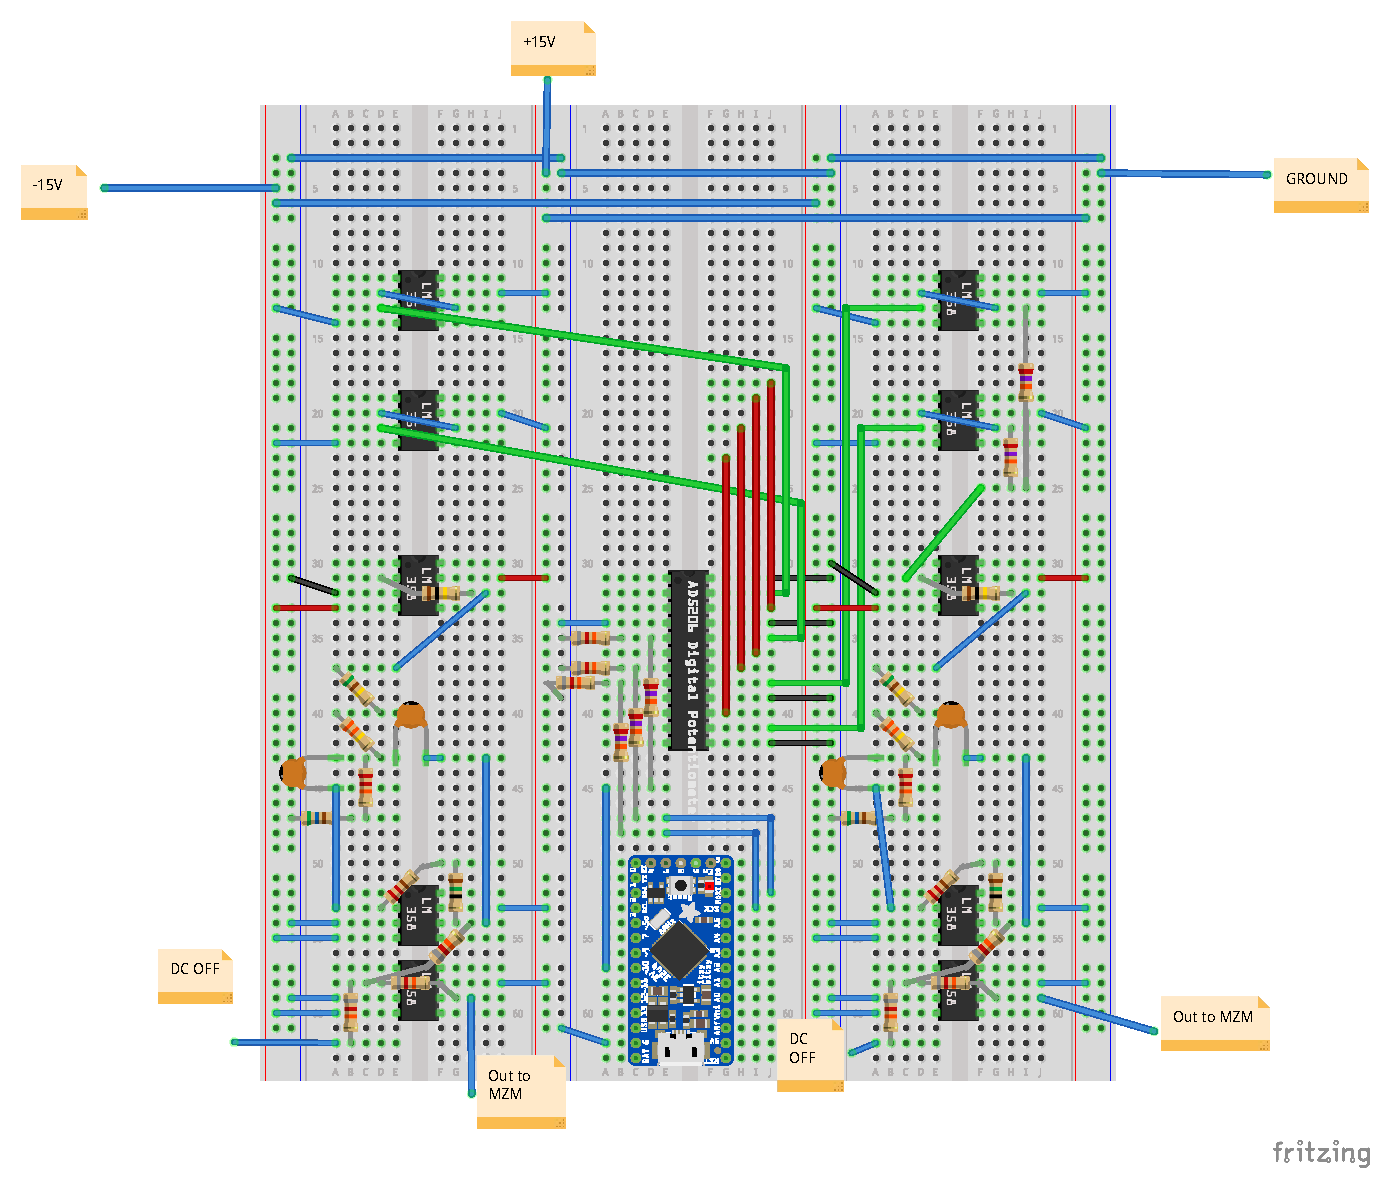
\includegraphics[width=\textwidth]{figs/bb.pdf}
        \caption{The electronic part of the optoelectronic oscillator}
        \label{circuitdiag}
    \end{figure}

    \begin{figure}[]
        \centering
        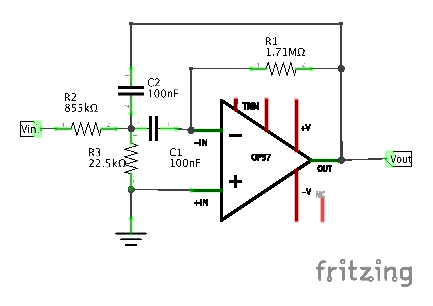
\includegraphics[]{figs/bpfilt.pdf}
        \caption{The bandpass filter, with (nominal) component values}
        \label{bpfiltdiag}
    \end{figure}

    \subsection{The AD5206 Digital Potentiometer}

    The AD5206 digital potentiometer is---by far---the most finicky part of the circuit. I accidentally fried a number of these chips while trying to determine how they worked, and I know Yunjia faced similar problems. A brief summary application note on these devices I wrote earlier in the summer:

    \begin{itemize}
        \item The AD5206 behaves like six mechanical potentiometers.
        \item Each potentiometer has three terminals (A,B, and W), just like a mechanical.
        \item These potentiometers are (to the best of my knowledge) completely isolated---I did not observe any leakage between them.
        \item There are two power terminals on the chip: $V_{\text{SS}}$ and $V_{\text{DD}}$.
        \item These terminals are subject to the constraints that
        \begin{equation*}
            V_{\text{SS}} \leq 0 \leq V_{\text{DD}}
        \end{equation*}
        and
        \begin{equation*}
            |V_{\text{DD}}| + |V_{\text{SS}}| \leq 5.5V
        \end{equation*}
        \item The potentials of all three wiper terminals MUST be between $V_\text{SS}$ and $V_\text{DD}$:
        \begin{equation*}
            V_\text{SS} \leq \{A,B,W\} \leq V_\text{DD}
        \end{equation*}
        \item If this condition is not met, the response is nonlinear, and signals are distorted.
    \end{itemize}
    \subsubsection*{Monopolar Mode}
        These potentiometers are usually used in (and most online resources assume) monopolar mode
        \begin{itemize}
            \item In this mode, $V_{\text{SS}} = 0V = \text{GND}$, and $V_{\text{DD}} = 5V$.
            \item This is very convenient, since the logic output of most microcontrollers (e.g. Arduino) is $5V$, so no step-down is needed.
            \item However, because of the voltage bounds mentioned above, this means we can't send zero-offset AC signals (like we're working with here) through the digipot
            \item We could add an offset using an opamp, but that makes scaling very difficult, and adds unnecessary noise.
        \end{itemize}
    \subsubsection*{Bipolar Mode}
         Instead, we can operate in bipolar mode, where $V_{\text{SS}} < 0$. Some considerations in this mode:
        \begin{itemize}
            \item The potential bounds still apply. If we power the digipot with $\pm 2.5V$, the signal must fall within those bounds as well. This should not be a problem, since our signal should be within the $\pm1V$ envelope.
            \item The logic voltage must be within $0.3V$ of $V_\text{DD}$ (or specifically, when $V_\text{DD} = 3V$, the logic must be between $2.6V$ and $3.3V$, as per the datasheet).
            \item Logic low is still ground.
            \item I am driving the chip with an Adafruit ItstBitsy arduino, which uses 3.3V logic. I have implemented voltage dividers on each data channel to bring the signal to the required 2.5V.
        \end{itemize}
    \subsubsection*{Communication}
        \begin{itemize}
            \item We communicate with the potentiometer using SPI (serial peripheral interface).
            \item To set a resistance:
            \begin{itemize}
                \item Drive the CS (chip select) pin low
                \item Write the address as a single byte, MSB first. Because valid addresses are $0-5$ (zero-indexed), the word will look like \texttt{0b00000101} (for address 5).
                \item In Arduino, this can be done with \texttt{SPI.transfer(channel)}, where channel is in the range $0-5$.
                \item Then write the desired potentiometer value as a single byte, ranging from 0 (minimum resistance) to 255 (maximum resistance). In theory, the output resistance at step $n$ will be
                \begin{equation*}
                    R_\text{out} = (n/255)\cdot \SI{50}{\kilo\ohm}
                \end{equation*}
                Experimental response curves are detailed below.
                \item Drive the CS pin high.
                \item The code used on the Arduino is in the associated Github repository.
            \end{itemize}
        \end{itemize}

        \subsubsection*{Characterizing and Using the Chip}
        \begin{itemize}
            \item Be careful when testing the chip. A natural instinct would be to test the chip by hooking it up to a multimeter and sweeping through the various settings. However, multimeters (typically) work by appling a $5V$ potential difference, and measuring the associated current. Since (in bipolar mode) $5V$ is outside of the $[V_{ss}, V_{dd}]$ range, this will kill the chip. I fried at least two chips doing this.
            \item There are two ways we can use the chip. In rheostat mode, we use the chip directly as a variable resistor that can be digitally tuned, such as by using it as one of the resistors in a summing amplifier. In the potentiometer mode, we use the chip as a programmable voltage divider---essentially, a variable gain amplifier with a gain between 0 and 1.
            \begin{itemize}
                \item In rheostat mode, we need to worry about overcurrent. Assuming a 1V signal (broadly typical), and that the output is tied to ground (which, with the summing amplifier design, is true), the current flowing through the chip at the minimum resistance of $\SI{50}{\ohm}$ is
                \begin{equation*}
                    I = \frac{V}{R} = \SI{0.02}{\A} = \SI{20}{\milli\A}
                \end{equation*}
                Given that the absolute maximum continuous current should not exceed $\SI{2.5}{\milli\A}$, this is bad. I killed a chip this way too (it got very warm).
                \item In potentiometer mode, terminal B is tied to ground, and terminal A is tied to $V_{in}$. The output voltage on the wiper is then
                \begin{equation*}
                    V_{out} = \frac{n}{255}V_{in}
                \end{equation*}
                where $n$ is the digital input.

                The other main advantage of potentiometer mode is reduced temperature dependence. The digital potentiometer (and all potentiometers) has a relatively large temperature coefficient, so the actual resistance/tick value changes with temperature. However, in the voltage divider equation, multiplying all resistances by some factor does not change the output voltage---so, by using this mode, we do not have to account for temperature in our circuit.
            \end{itemize}
        \end{itemize}

        \subsubsection*{Response curves}
        \begin{tabular}{lll}
            \toprule
            Potentiometer & Base resistance ($\Omega$) & Response ($\Omega/\text{tick}$) \\ \midrule
            Ideal & $50$ & $196.1$ \\
            R1 & $30.3$ & $202.6$ \\
            R2 & $39.5$ & $202.3$ \\
            R3 & $39.9$ & $202.1$ \\
            R4 & $42.0$ & $202.1$ \\
            R5 & $10.9$ & $202.6$ \\
            R6 & $27.4$ & $202.4$ \\\bottomrule
        \end{tabular}\vspace{1em}

        \noindent These resistors have a small (near-negligible) wiper resistance, and a slightly higher maximum resistance than advertised. The typical maximum resistance was about $\SI{51.5}{\kilo\ohm}$. No statistically significant nonlinearity was observed.

        \subsubsection*{Other notes}
        \begin{itemize}
            \item It may be worthwhile to look into other digital potentiometers, especially if this one breaks or burns out. As far as I can tell, Analog Devices (AD) is the largest and most reputable manufacturer of these chips.
            
            One chip I was looking at was the AD5263, which only has four channels (instead of the six found on the AD5206), but can be powered by a $\pm5$V supply (and therefore 5V logic).

            \item Unfortunately, Analog seem to have discontinued all DIP-packaged chips, so any new model of potentiometer (or replacements for the existing one, if it breaks) means dealing with SMD parts and breakout boards.
            
            \item It may be worthwhile to look into replacing the digital potentiometer with variable gain amplifiers, especially since the potentiometer/voltage follower combo essentially act as a variable gain amplifier anyways.
        \end{itemize}

        \section{Utilities}
        \subsection{\code{combine_figs.py}}
        This is a useful little script for combining multiple figures together on one page for printing or easy comparison. To use:
        \begin{lstlisting}
            python scripts/combine_figs.py <outfile.pdf> <fig1> <fig2> ...
        \end{lstlisting}
        where all the figures are in the same directory as \code{outfile.pdf}. This thing uses LaTeX behind the scenes, so if things go south, that's probably the place to look.

    \bibliography{documentation}{}
    \bibliographystyle{plain}
\end{document}